\section{General Innovation Theory}

\subsection{Basic Terms}
\begin{itemize}
	\item \textbf{Creativity}: a state of mind which leads to inventive or innovative thinking.
	\item \textbf{Invention}: e.g., a new algorithm, new use of data, or program.
	\item \textbf{Innovation}: creative atc and invention carried into wider use, leading to substantial kinds of change. Innovation implies the successful use exploration of new ideas.
\end{itemize}

\subsection{A combination of Activities}
\begin{itemize}
	\item \textbf{Innovation = invention + exploitation + diffusion}.
	\item \textbf{Invention}: The creative act or process and its result.
	\item \textbf{Exploitation}: Commercial development and adaptation to practical situations.
	\item \textbf{Diffusion}: Adoption by a wider audience.
\end{itemize}

\subsection{Dimensions of Innovation}
\begin{figure}[H]
	\centering
	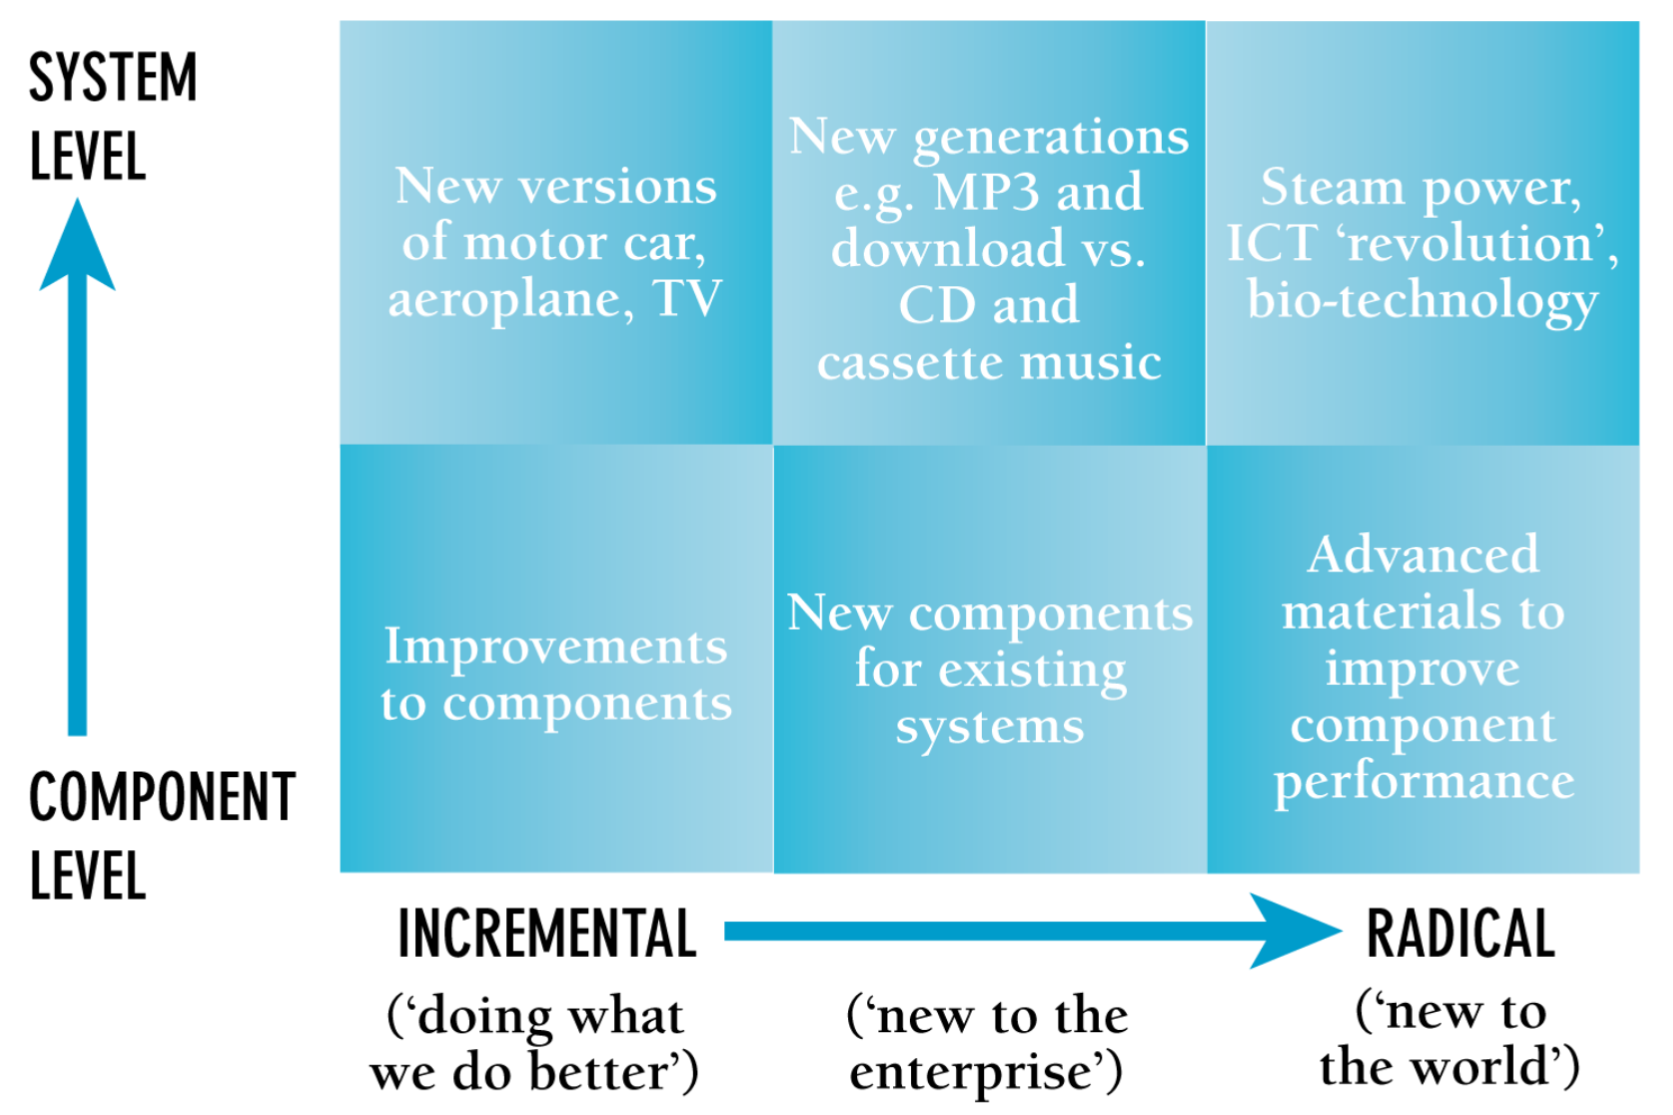
\includegraphics[width=0.75\textwidth]{Dimensions of Innovation.png}
	\caption{Tidd, J., Bessant, J. R., and Pavitt, K. 2005 Managing innovation: integrating technological, market and organization change. Wiley.}
\end{figure}

\subsection{Innovation Space}
\begin{figure}[H]
	\centering
	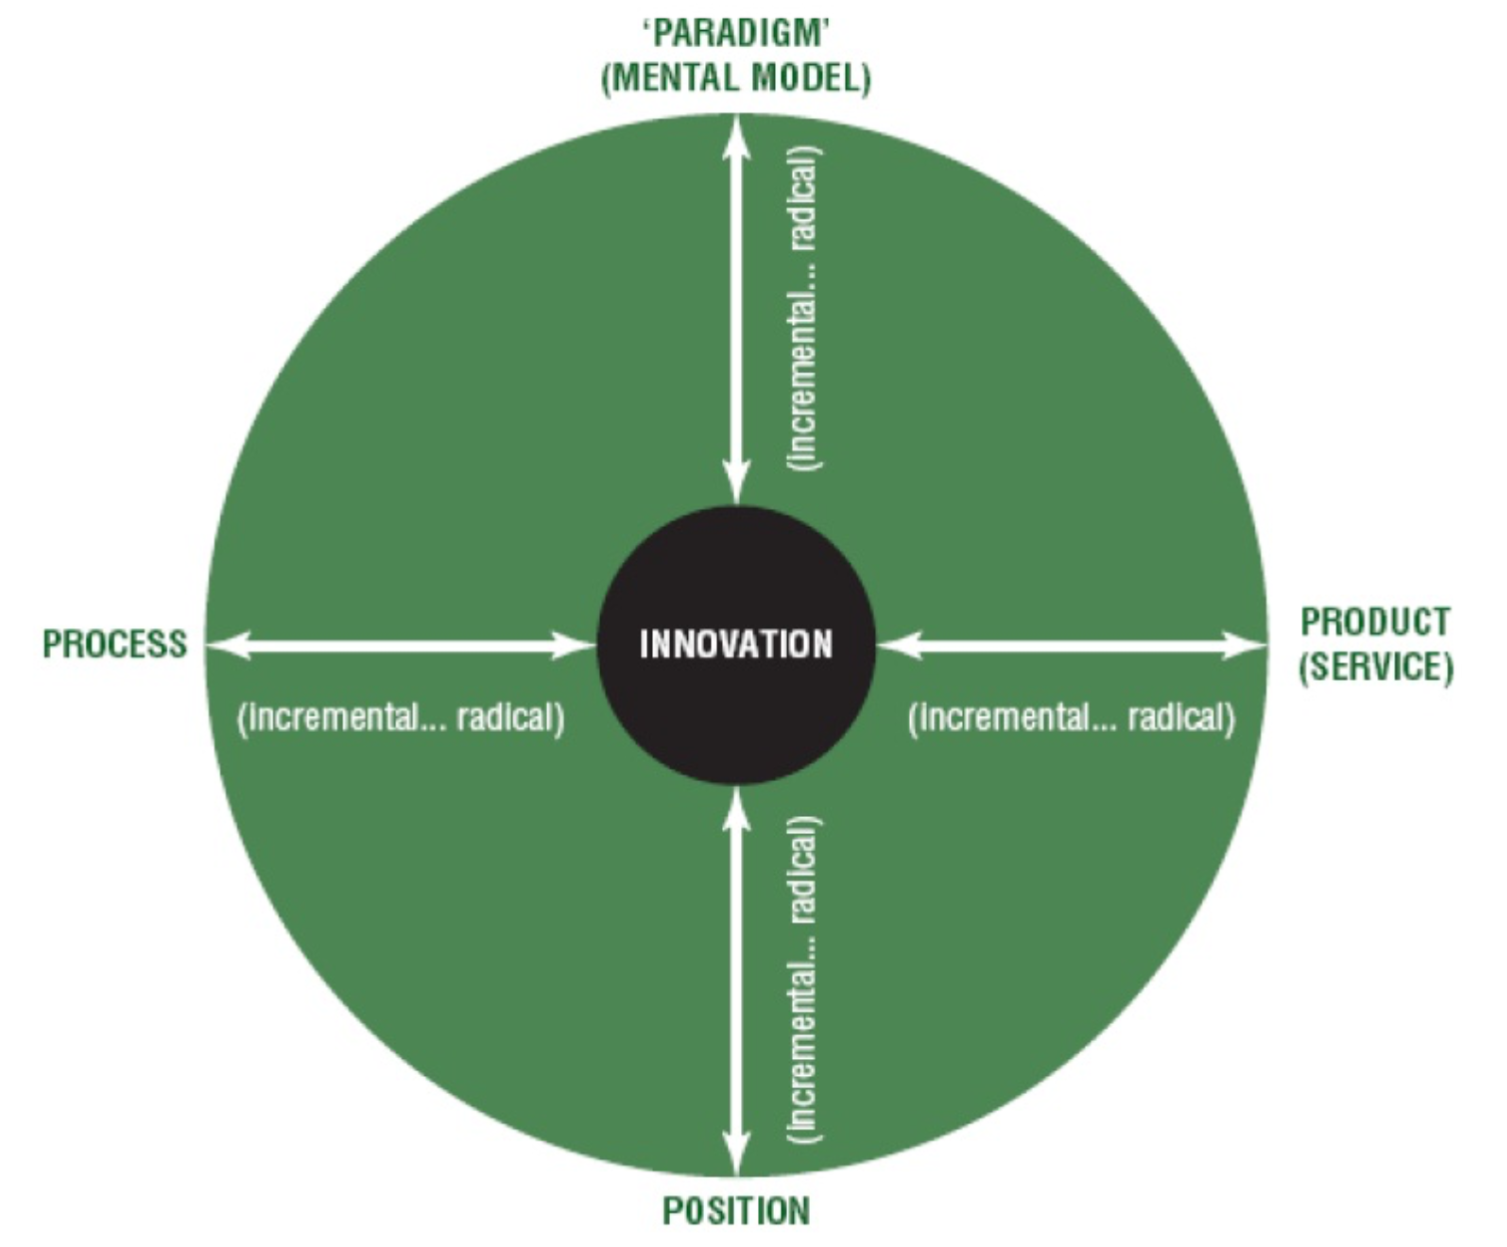
\includegraphics[width=0.75\textwidth]{Innovation Space.png}
	\caption{Tidd, J., Bessant, J. R., and Pavitt, K. 2005 Managing innovation: integrating technological, market and organization change. Wiley.}
\end{figure}

\subsection{Novelty: Levels of Innovation (Altshuller)}
\begin{itemize}
	\item \textbf{Level 1}: Routine design problems solved by methods well known with the specialty - usually no invention needed.
	\item \textbf{Level 2}: Minor improvements to an existing system using methods known within the industry.
	\item \textbf{Level 3}: Fundamental improvement to an existing system using methods known outside the industry.
	\item \textbf{Level 4}: A new generation of a system that entails a new principle for performing the system's primary functions - solutions are found more often in science than technology.
	\item \textbf{Level 5}: A rare scientific discovery or pioneering invention of an essentially new system.
\end{itemize}

\begin{figure}[H]
	\centering
	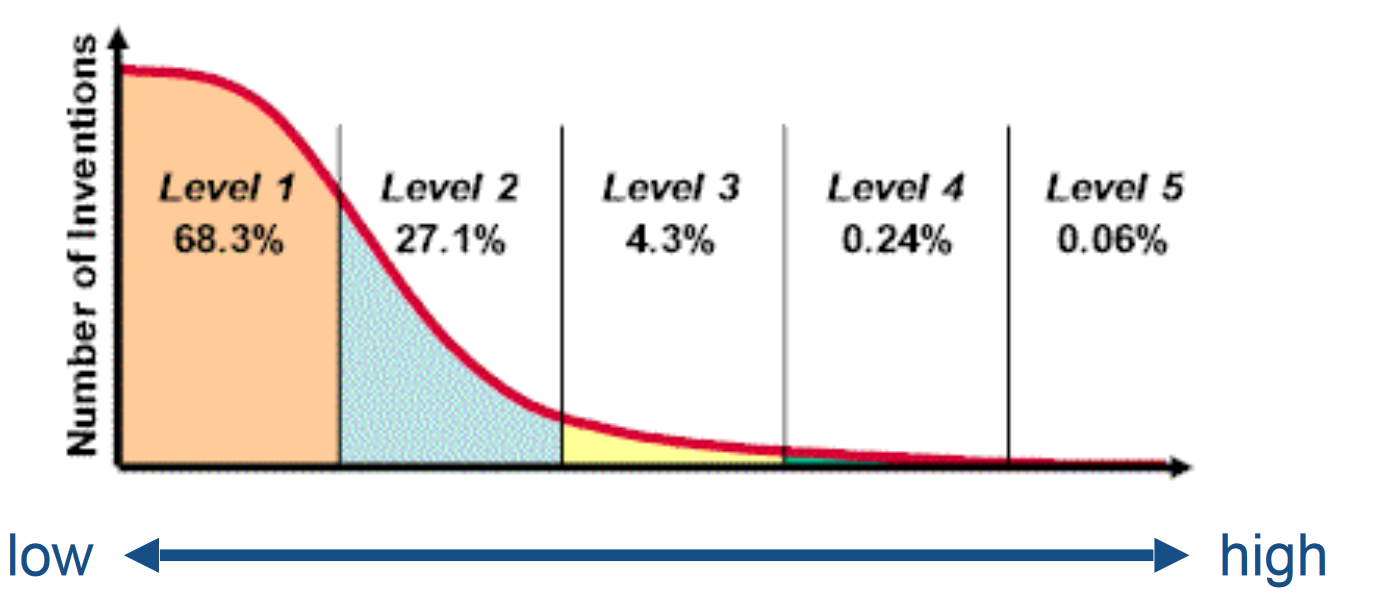
\includegraphics[width=0.75\textwidth]{Levels of Innovation.png}
	\caption{Jeremy Rose}
\end{figure}

\subsection{Hierarchies of Technical Systems (Altshuller)}
\begin{figure}[H]
	\centering
	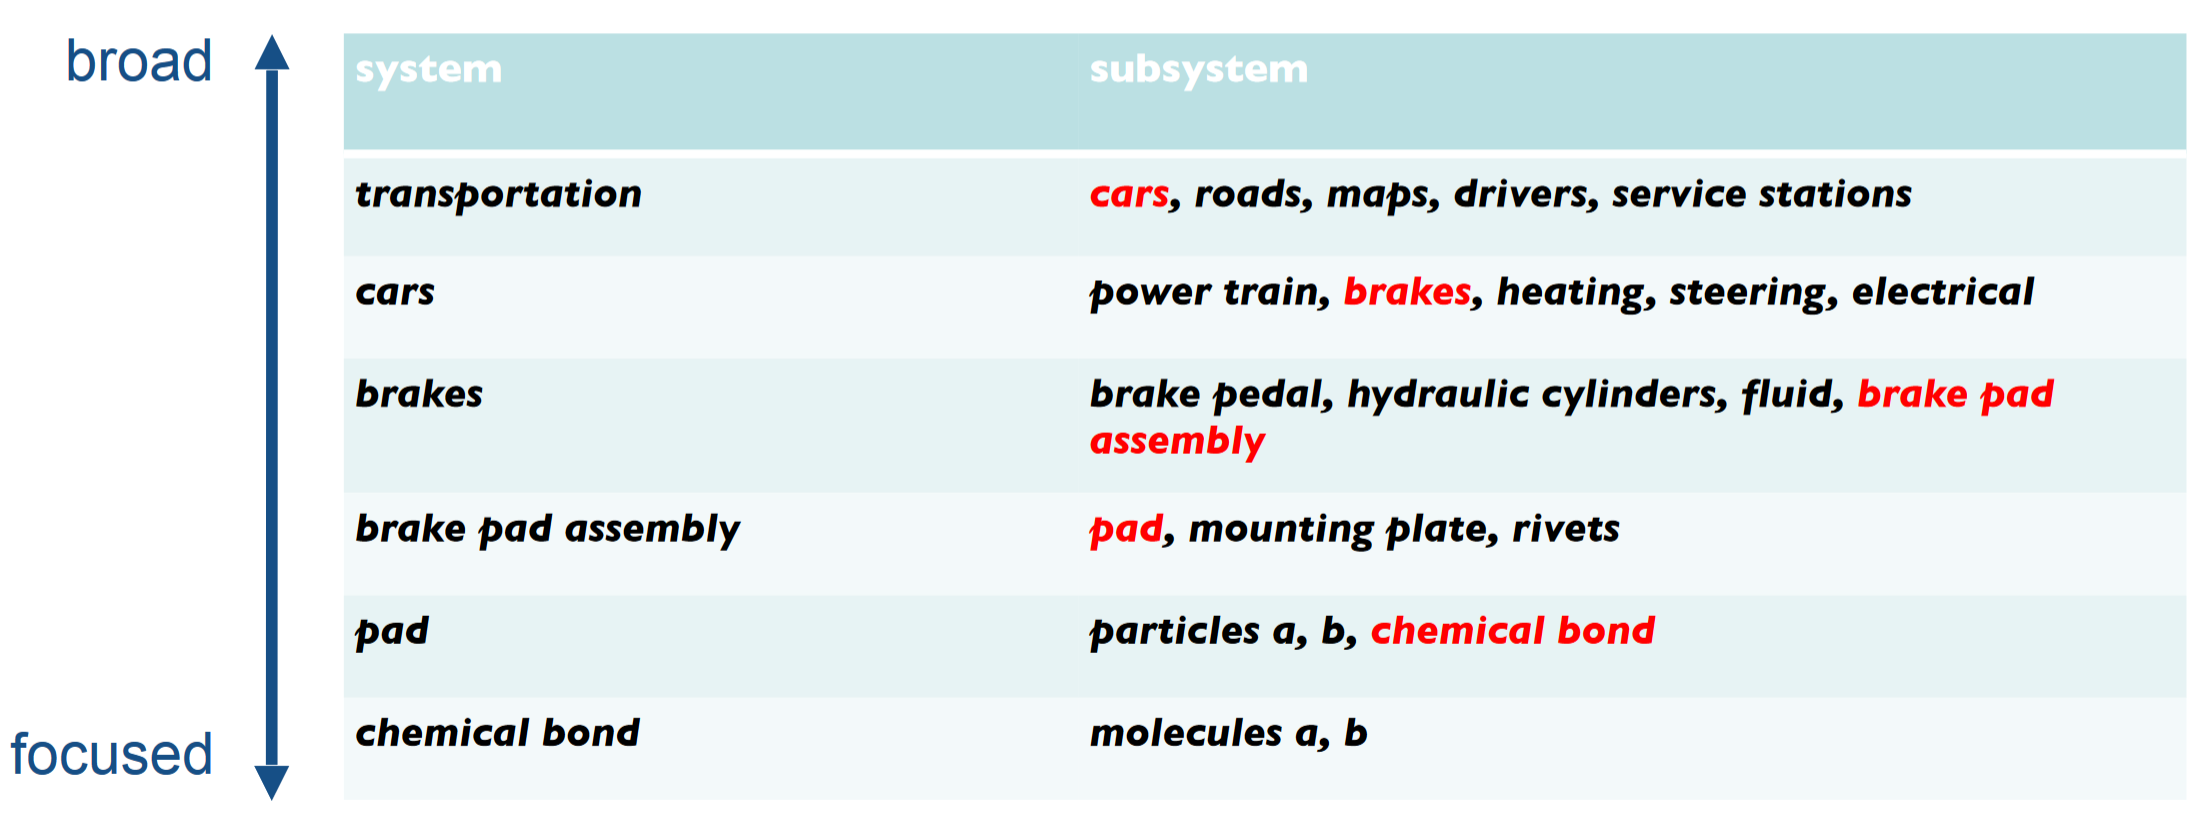
\includegraphics[width=0.9\textwidth]{Hierarchies of Technical Systems.png}
	\caption{Jeremy Rose}
\end{figure}

\subsection{Incremental and Radical Innovation}
\begin{figure}[H]
	\centering
	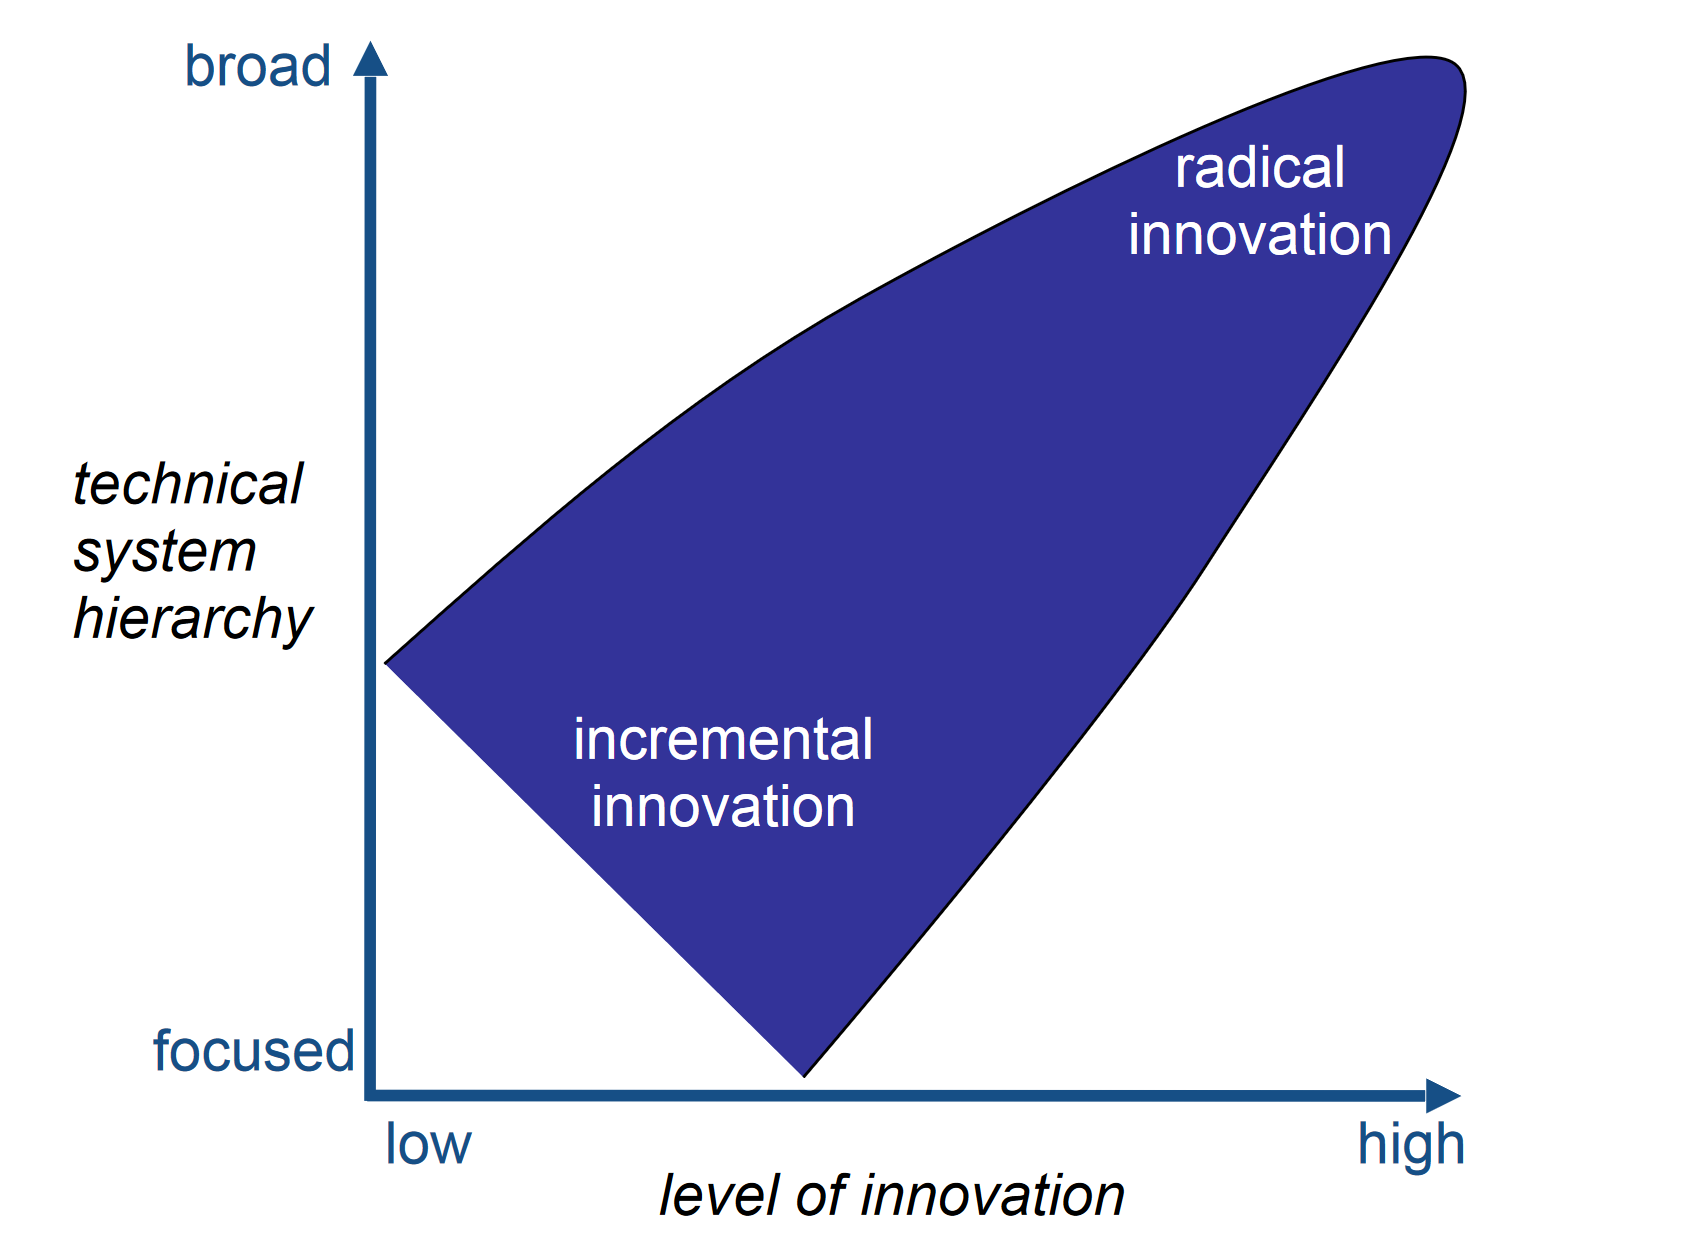
\includegraphics[width=0.75\textwidth]{Incremental and Radical Innovation.png}
	\caption{Jeremy Rose}
\end{figure}